Campuses that wish to use GPS to unlock puzzles should provide
a \textbf{Campus Map} designating several possible locations players
may visit during the game. Each location should be labeled with
a letter/number pair matching the sectors of the \textbf{Galaxy Chart}.
(If only eight locations are available, each location can be associated
with two sectors. Note that only sectors 
A1, A3, B3, C1,
C2, C3, D2 are used.)

For example:

\begin{center}
  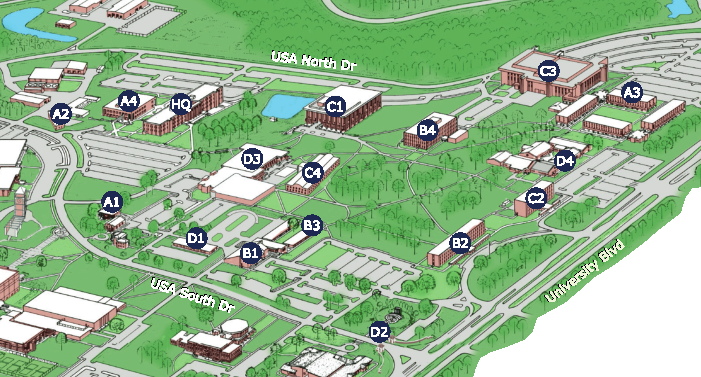
\includegraphics[width=\linewidth]{assets/south-map}
\end{center}

\begin{multicols}{2}
  \begin{itemize}
    \item A1: Alumni Hall
    \item A2: Archaeology Museum
%    \item Central Services Admin Building % 30.69875, -88.17618
    \item A3: Charles M. Baugh Biomedical Library
    \item A4: Chemistry Building
    \item B1: Computer Services Center
    \item B2: F.P. Whiddon Administration Building % 30.6954, -88.17492
%    \item Glass Arts Building % 30.69708, -88.17642
%    \item Humanities Building
    \item B3: Innovation in Learning Center
    \item B4: Life Sciences Building
    \item C1: Marx Library
    \item C2: Math. Sciences and Physics Bldg. 
    \item C3: Medical Sciences Building
    \item C4: Meisler Hall % 30.69595, -88.17747
%    \item Mobile Townhouse 
    \item D1: Student Health Center
    \item D2: Tholos of Delphi Replica
    \item D3: USA Student Center
    \item D4: Visual Arts Complex
  \end{itemize}
\end{multicols}

Team Headquarters are located in the Humanities
Building (labeled HQ on the map).
Players will not need to cross USA South Dr, USA North Dr, or University Blvd.
